% dc_bias_single_phase_transformers.tex
% Componente continua nei trasformatori monofase alimentati da un inverter V/f in anello aperto: perche' una piccola
% corrente continua satura il nucleo, livelli tollerabili, sorgenti di errore dell'inverter, e compensazione della
% continua agendo solo sulle componenti alpha-beta del vettore spaziale di tensione (anello lento PI aggiunto al V/f).
% Template pwr-control (AAA_template_latex_settings); numeri e figure: dc_bias_analysis.py (python3, numpy, matplotlib).
% Compilazione: pdflatex dc_bias_single_phase_transformers.tex (tre volte, per i riferimenti).
% Rev. 00 - ottobre 2026 - prima emissione
\documentclass[10pt,a4paper]{scrartcl}
\PassOptionsToPackage{main=italian}{babel}   % settings.tex carica babel con [british]: l'italiano diventa la lingua principale
% ===================== PACKAGES =====================
\usepackage[british]{babel}
\usepackage[tmargin=1in, bmargin=1in, lmargin=0.75in, rmargin=0.75in]{geometry}
\usepackage[dvipsnames,table]{xcolor}  % prima di tikz, listings, ecc.

\usepackage{tikz}
\usepackage{graphicx}
\usepackage{pgfplots}
\pgfplotsset{width=12cm, compat=1.9}
\usepackage{setspace}
\usepackage{chemmacros}
\usepackage{chemfig}
\usepackage{esint}
\usepackage{tabularray}
\usepackage{makeidx}
\usepackage{epstopdf}
\usepackage{amssymb}
\usepackage{mathrsfs}
\usepackage{bm}
\usepackage{amsmath}
\usepackage{enumitem}
\usepackage[english]{varioref}
\usepackage{lipsum}
\usepackage{fancyhdr}
\usepackage{float}
\usepackage{empheq}
\usepackage[framemethod=tikz]{mdframed}
\numberwithin{equation}{section}
\usepackage{eso-pic}
\usepackage{calc}
\usepackage{nccmath}
\usepackage{caption}
\usepackage{subcaption}
\usepackage{gensymb}
\usepackage{amsfonts, amsthm, epsfig, epstopdf, titling, url, array}
\usepackage{tabularx}
\usepackage{makecell}
\usepackage{booktabs}
\usepackage{array}
\usepackage{siunitx}
\sisetup{input-digits=0123456789\pi}
\usepackage[symbol]{footmisc}
\usepackage{multicol}
\usepackage{boondox-cal}
\usepackage{blindtext}
\usepackage{changepage}
\usepackage{nomencl}
\usepackage{hyperref}
\usepackage{xurl}
\usepackage{ragged2e}
\usepackage[version=4]{mhchem}  % ← conflitto di opzioni
\usepackage{longtable}
\usepackage{chemformula}
\usetikzlibrary{arrows.meta,positioning,calc}

% ===================== SI UNITS =====================
\DeclareSIUnit\atm{atm}
\DeclareSIUnit{\var}{var}
\DeclareSIUnit{\pu}{p.u.}


% ===================== MATH OPERATORS =====================
\DeclareMathOperator{\rank}{rank}
\DeclareMathOperator{\atantwo}{atan2}
\DeclareMathOperator{\spn}{span}

% ===================== COMMANDS =====================
\newcommand{\abs}[1]{\left|#1\right|}
\newcommand{\sign}{\text{sign}}
\newcommand{\centered}[1]{\begin{tabular}{@{}l@{}} #1 \end{tabular}}

% ===================== COLORS =====================
\definecolor{mycolor1}{rgb}{0.97, 0.97, 0.97}
\definecolor{mycolor2}{rgb}{0.97, 0.97, 0.97}
\definecolor{tableShade}{gray}{0.9}

% ===================== THEOREM ENVIRONMENTS =====================
\theoremstyle{it}
\newtheorem{defn}{Definition}[section]
\newtheorem{assumption}{Assumption}[section]
\newtheorem{thm}{Theorem}[section]
\newtheorem{lemma}{Lemma}[section]
\newtheorem{corollary}{Corollary}[section]
\theoremstyle{definition}
\newtheorem{example}{Example}[section]

% ===================== CUSTOM ENVIRONMENTS =====================
\newenvironment{myitemize_1}{
	\begin{itemize}[topsep=0pt]
		\setlength{\topsep}{2pt}
		\setlength{\itemsep}{2pt}
		\setlength{\parskip}{2pt}
		\setlength{\parsep}{2pt}
	}{\end{itemize}}

\newmdenv[
innerlinewidth=0.5pt,
roundcorner=4pt,
backgroundcolor=mycolor2,
linecolor=mycolor1,
innerleftmargin=6pt,
innerrightmargin=6pt,
innertopmargin=6pt,
innerbottommargin=6pt
]{mybox}

% ===================== TABLE COLUMN TYPES =====================
\newcolumntype{Y}{>{\hsize=2\hsize}X}
\newcolumntype{Z}{>{\centering\arraybackslash\hsize=0.857\hsize}X}

% ===================== SECTION DEPTH =====================
\setcounter{secnumdepth}{3}
\setcounter{tocdepth}{3}

% ===================== PAGE STYLE =====================
\setlength{\headheight}{20pt}
\setlength{\headsep}{20pt}

\pagestyle{fancy}
\fancypagestyle{firstpage}{\rhead{}}
\fancyhead[L]{\slshape\nouppercase{\leftmark}}
\chead{}
\rhead{\includegraphics[height=0.75cm]{../../AAA_template_latex_settings/pwr-control_logo_doc.png}}
\lfoot{\href{http://www.pwr-control.com}{pwr-control.com}}
\cfoot{-\ \thepage\ -}
\rfoot{\textit{}}
\renewcommand{\headrulewidth}{0.4pt}
\renewcommand{\footrulewidth}{0.4pt}


\geometry{
	a4paper,
	top    = 2.5cm,
	bottom = 3.0cm,
	left   = 2.5cm,
	right  = 2.5cm
}

\hypersetup{
	colorlinks = true,
	urlcolor   = blue,
	linkcolor  = black,
	citecolor  = black
}

\pagenumbering{gobble}
% il documento sta tre livelli sotto la radice del repository: percorso del logo di settings.tex corretto qui
\rhead{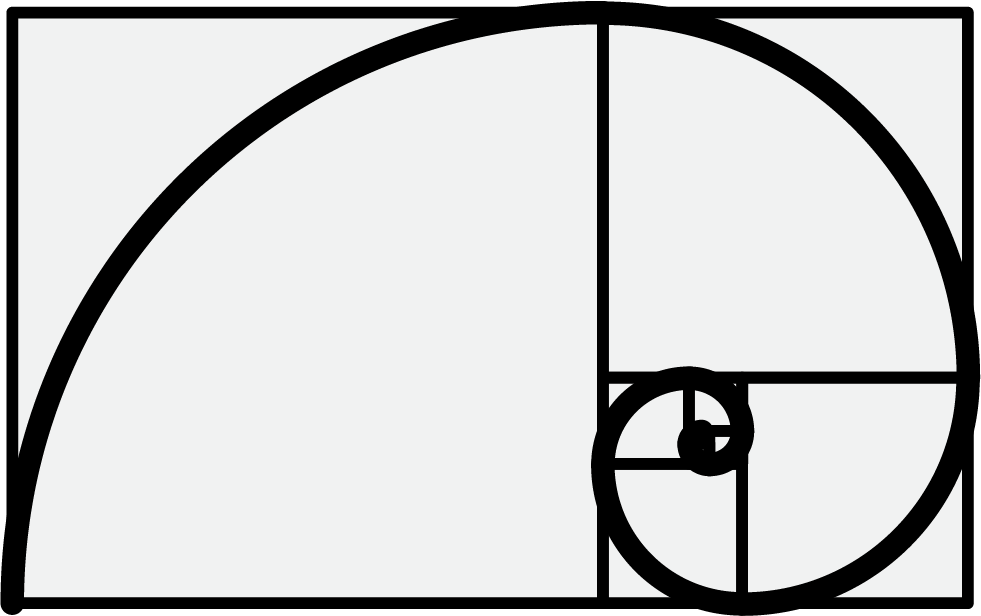
\includegraphics[height=0.75cm]{../../../AAA_template_latex_settings/pwr-control_logo_doc.png}}
\rfoot{\small Rev.~00}
\geometry{left=2.0cm, right=2.0cm}
\newcolumntype{R}[1]{>{\RaggedRight\arraybackslash}p{#1}}
\usetikzlibrary{shapes.geometric}

\sisetup{output-decimal-marker={,}, per-mode=symbol, range-phrase={--}, range-units=single, list-final-separator={ e },
         exponent-product=\cdot}
\DeclareSIUnit{\VA}{VA}
\setlist{nosep}
\setlength{\parindent}{0pt}
\setlength{\parskip}{3pt}
\allowdisplaybreaks

% --- abbreviazioni (non si usano \dd, \abs, \norm, \vec, \grad, \tr, \var, \order, \dv, \wr: occupate da physics/LaTeX) ---
\newcommand{\jj}{\mathrm{j}}
\newcommand{\ee}{\mathrm{e}}
\newcommand{\dif}{\mathrm{d}}
\newcommand{\code}[1]{\texttt{#1}}
\newcommand{\Ts}{T_s}
\newcommand{\Tuno}{T_1}
\newcommand{\Lm}{L_m}
\newcommand{\Lsat}{L_{sat}}
\newcommand{\Linc}{L_{inc}}
\newcommand{\lamhat}{\hat\lambda}
\newcommand{\lams}{\lambda_s}
\newcommand{\lamdc}{\lambda_{dc}}
\newcommand{\Idc}{I_{dc}}
\newcommand{\Izero}{I_0}
\newcommand{\Izeropk}{\hat I_0}
\newcommand{\ab}{\alpha\beta}
\newcommand{\Iab}{I_{\ab}}
\newcommand{\Eab}{E_{\ab}}
\newcommand{\dvab}{\Delta v_{\ab}}
\newcommand{\kp}{k_p}
\newcommand{\ki}{k_i}
\newcommand{\Udc}{U_{dc}}
\renewcommand{\Re}{\operatorname{Re}}
\renewcommand{\Im}{\operatorname{Im}}

% =============================================================
%  DATI DEL DOCUMENTO (frontespizio: AAA_template_latex_settings/titlepage.tex)
% =============================================================
\newcommand{\DocCategory}{Nota tecnica}
\newcommand{\DocField}{Elettronica di potenza e sistemi di controllo}
\newcommand{\DocTitle}{%
	{\fontsize{19}{23}\selectfont\bfseries Componente continua nei trasformatori monofase \\[6pt] alimentati da un inverter V/f in anello aperto:} \\[12pt]
	{\fontsize{15}{20}\selectfont\bfseries effetti, livelli tollerabili, sorgenti di errore \\[6pt] e compensazione sulle componenti $\alpha\beta$ della tensione}
}
\newcommand{\DocSubtitle}{Tre trasformatori monofase senza traferro su un inverter IGBT a due livelli in V/f: \\[6pt] quanta continua tollerano, quanta ne produce l'inverter, e come annullarla \\[6pt] con un anello lento che sposta solo $v_\alpha$ e $v_\beta$ del vettore spaziale di riferimento}
\newcommand{\DocAuthor}{Davide Bagnara}
\newcommand{\DocRevision}{00}
\newcommand{\DocDate}{Ottobre 2026}
\newcommand{\DocAbstract}{%
Un inverter trifase IGBT a due livelli in controllo V/f in anello aperto alimenta tre trasformatori monofase da \SI{1.7}{M\VA} senza traferro. La nota stima quanta corrente continua i trasformatori tollerano (l'ordine della corrente a vuoto $\Izero \approx \SI{7}{A}$: oltre, saturazione a semionda, impulsi magnetizzanti di decine di volte $\Izero$, seconda armonica, rumore, riscaldamento delle parti strutturali) e quanta ne produce l'inverter (anello di \SIrange{2}{4}{m\ohm} in continua, \SIrange{50}{150}{mV} di errore fra i rami, cioè \SIrange{15}{50}{A}: la saturazione è l'esito atteso). Il V/f resta in anello aperto e si aggiunge un anello lento sulla sola continua: con primari a stella e neutro isolato le tre correnti continue hanno somma nulla e dipendono dalle sole componenti $\alpha\beta$ dell'errore di tensione, quindi la trasformata di Clarke della media su un periodo delle tre correnti dà il vettore $\Iab$ e un PI per asse aggiunge l'offset $\dvab$ al vettore spaziale di riferimento. L'impianto in continua è quasi un integratore ($\Lm/R \approx \SI{100}{s}$ in zona lineare, pochi millihenry in saturazione): il solo integratore non basta, il termine proporzionale è una resistenza virtuale necessaria e il suo massimo è fissato dal nucleo saturo. Con $\kp = \SI{50}{m\ohm}$ un gradino di \SI{67}{mV} dà al massimo \SI{0.9}{A} invece di \SI{23}{A} e un nucleo già saturo è desaturato in pochi secondi. Il residuo è l'offset dei sensori: il modo comune è rigettato, l'auto-azzeramento e i sensori flux-gate riducono il resto, e la regolazione della seconda armonica, insensibile all'offset, usa la stessa struttura $\alpha\beta$. Uno script Python riproduce ogni numero e figura.
}
\newcommand{\RevisionHistory}{%
	00 & Ottobre 2026 & Prima emissione. & \DocAuthor \\
}
\newcommand{\MetaLabelA}{Repository}
\newcommand{\MetaValueAUrl}{https://github.com/pwr-control/repositories-documentation.git}
\newcommand{\MetaValueALabel}{repositories-documentation.git (research/power\_electronics)}
\newcommand{\MetaLabelB}{Strumenti}
\newcommand{\MetaValueB}{Python 3 (\code{dc\_bias\_analysis.py}: numpy, matplotlib)}

\begin{document}
% =============================================================
%  pwr-control LaTeX template - FRONTESPIZIO
%
%  Da richiamare come prima istruzione dopo \begin{document}:
%      \input{../../AAA_template_latex_settings/titlepage}
%
%  Il documento deve definire prima di \begin{document}:
%      \DocCategory   categoria del documento
%      \DocField      area tecnica
%      \DocTitle      titolo (una o due righe)
%      \DocSubtitle   sottotitolo
%      \DocAuthor     autore/i, separati da virgola
%      \DocRevision   numero di revisione corrente (es. 00)
%      \DocDate       data della revisione corrente
%      \DocAbstract   abstract
%      \RevisionHistory  righe della tabella di revisione, nel formato
%                        Rev. & Date & Description & Authors \\
%      \MetaLabelA \MetaValueAUrl \MetaValueALabel
%      \MetaLabelB \MetaValueB
% =============================================================

\providecommand{\DocCategory}{Technical Research Report}
\providecommand{\DocField}{Power Electronics and Control Systems}
\providecommand{\DocSubtitle}{}
\providecommand{\DocRevision}{00}
\providecommand{\DocAbstract}{}
\providecommand{\RevisionHistory}{%
	\DocRevision & \DocDate & First issue. & \DocAuthor \\
}

\titlepage

% ---- Intestazione centrata ----
\begin{center}
	{\Large\scshape \DocCategory}\\[8pt]
	{\large\scshape \DocField}
\end{center}

\vspace{30pt plus 4pt minus 14pt}
\noindent\rule{\linewidth}{0.8pt}

% ---- Titolo ----
\begin{center}
	\DocTitle
\end{center}

\vspace{4pt}
\noindent\rule{\linewidth}{2.2pt}

% ---- Sottotitolo ----
\begin{center}
	\begin{onehalfspace}
		{\large\itshape \DocSubtitle}
	\end{onehalfspace}
\end{center}

% ---- Authors / Revision / Date ----
\vspace{30pt plus 4pt minus 14pt}

\noindent
\begin{minipage}[t]{0.46\linewidth}
	\raggedright
	\textbf{Authors:}\\[2pt]
	\DocAuthor
\end{minipage}%
\hfill
\begin{minipage}[t]{0.22\linewidth}
	\centering
	\textbf{Revision:}\\[2pt]
	\DocRevision
\end{minipage}%
\hfill
\begin{minipage}[t]{0.30\linewidth}
	\raggedleft
	\textbf{Date:}\\[2pt]
	\DocDate
\end{minipage}

\vspace{10pt}
\noindent\rule{\linewidth}{0.8pt}

% ---- Abstract ----
\vspace{24pt plus 4pt minus 12pt}

\begin{center}
	\begin{minipage}{0.88\linewidth}
		\footnotesize
		\begin{onehalfspace}
			\textbf{Abstract:} \DocAbstract
		\end{onehalfspace}
	\end{minipage}
\end{center}

\vfill

% ---- Revision history ----
\begin{center}
	\begin{minipage}{0.96\linewidth}
		\centering
		{\footnotesize\scshape Revision history}\\[6pt]
		{\footnotesize
			\begin{tabular}{@{}cl>{\raggedright\arraybackslash}p{0.36\linewidth}>{\raggedright\arraybackslash}p{0.28\linewidth}@{}}
				\toprule
				\textbf{Rev.} & \textbf{Date} & \textbf{Description} & \textbf{Authors} \\
				\midrule
				\RevisionHistory
				\bottomrule
			\end{tabular}}
	\end{minipage}
\end{center}

\vspace{18pt plus 4pt minus 10pt}

% ---- Metadati in fondo ----
\noindent
\begin{tabular}{@{} r @{\quad} l @{}}
	\textsc{\MetaLabelA:} & {\href{\MetaValueAUrl}{\MetaValueALabel}} \\[3pt]
	\textsc{\MetaLabelB:} & {\MetaValueB}       \\[3pt]
\end{tabular}

% =============================================================
%  Fine frontespizio
% =============================================================
\newpage
\pagenumbering{arabic}
\setcounter{page}{1}

\tableofcontents
\newpage
\begin{onehalfspace}

% =====================================================================================================
\section{Scopo e dati assunti}
\label{sec:scopo}

Un inverter trifase IGBT a due livelli in controllo V/f in anello aperto alimenta tre trasformatori monofase con nucleo senza traferro, uno per fase. Le domande sono due: quanta corrente continua tollerano i trasformatori e quanta ne può produrre un inverter in anello aperto. La risposta breve è che la continua tollerabile è dell'ordine della corrente a vuoto e che un inverter in anello aperto la supera facilmente. La nota riporta l'analisi (Sez.~\ref{sec:saturazione}--\ref{sec:energizzazione}) e progetta la compensazione (Sez.~\ref{sec:compensazione}): il V/f resta in anello aperto e un anello lento sulla sola componente continua sposta le componenti $\alpha$ e $\beta$ del vettore spaziale di tensione, le sole su cui l'inverter può agire.

I dati assunti sono in Tab.~\ref{tab:dati}; vanno confermati (Sez.~\ref{sec:aperti}). Tutte le cifre sono stime da principi primi: non si è usata alcuna misura né alcun rapporto di prova dei trasformatori reali. Ogni numero della nota è calcolato dallo script \code{dc\_bias\_analysis.py}, che riproduce anche le figure; cambiando i dati di testa dello script si riscalano tutte le stime.

\begin{table}[H]
\centering\small
\begin{tabular}{@{}R{5.0cm}R{10.5cm}@{}}
\toprule
\textbf{Voce} & \textbf{Valore assunto} \\
\midrule
Trasformatore & monofase, \SI{1.7}{M\VA}, nucleo senza traferro, uno per fase \\
Tensione nominale dell'avvolgimento primario $U_1$ & \SI{690}{V} (assunta): $I_n = S_n/U_1 = \SI{2464}{A}$ \\
Corrente a vuoto $\Izero$ & \SI{0.3}{\percent} di $I_n$ = \SI{7.4}{A} (tipico \SIrange{0.2}{0.5}{\percent} per questa taglia); picco $\Izeropk = \SI{10.5}{A}$ \\
Perdite nel rame & \SI{1}{\percent} a carico nominale, metà sul primario \\
Induzione & \SI{1.7}{T} di picco a tensione nominale, saturazione a \SI{2.0}{T} (lamierino a grani orientati) \\
Induttanza satura $\Lsat$ & \SI{0.2}{\pu} sulla base del trasformatore (nucleo d'aria dell'avvolgimento), cioè \SI{0.18}{mH} \\
Frequenza di uscita $f_1$ & \SI{50}{Hz} \\
Inverter & trifase a due livelli IGBT (classe \SI{2400}{A}), V/f in anello aperto, \SI{690}{V} concatenati in uscita \\
DC link $\Udc$ & \SI{1070}{V} ($m \approx \num{0.91}$ con SVM per \SI{690}{V} concatenati) \\
Frequenza di commutazione & \SI{1.25}{kHz} ($\Ts = \SI{800}{\micro s}$), rapporto di impulsi 25 a \SI{50}{Hz}, un aggiornamento per periodo \\
Tempo morto $t_d$ & \SI{5}{\micro s} \\
Collegamento dei primari & stella con neutro isolato (ipotesi; vedi Sez.~\ref{sec:aperti}) \\
\bottomrule
\end{tabular}
\caption{Dati assunti. Con i primari a stella sui \SI{690}{V} concatenati dell'inverter ogni avvolgimento vede \SI{398}{V}: se la tensione nominale dell'avvolgimento è \SI{398}{V} e non \SI{690}{V}, $I_n$ e $\Izero$ crescono di $\sqrt3$ e la resistenza e l'induttanza magnetizzante si riducono di tre volte (Sez.~\ref{sec:aperti}); la struttura dell'analisi e della compensazione non cambia.}
\label{tab:dati}
\end{table}

Dai dati assunti seguono le grandezze usate nel seguito: flusso concatenato di picco $\lamhat = \sqrt2\,U_1/\omega_1 = \SI{3.11}{Wb}$, flusso di saturazione $\lams = \lamhat\,B_{sat}/B_{max} = \SI{3.65}{Wb}$, margine $\lams - \lamhat = \SI{0.55}{Wb}$ (\SI{18}{\percent} di $\lamhat$), induttanza magnetizzante in zona lineare $\Lm = \sqrt2\,U_1/(\omega_1\Izeropk) = \SI{0.30}{H}$, impedenza di base $Z_b = U_1^2/S_n = \SI{0.28}{\ohm}$ e $\Lsat = \SI{0.2}{\pu} = \SI{0.18}{mH}$.

% =====================================================================================================
\section{Perché una piccola corrente continua satura il nucleo}
\label{sec:saturazione}

Una corrente continua nell'avvolgimento non si trasferisce al secondario: è interamente corrente magnetizzante. Con un nucleo senza traferro la riluttanza magnetizzante è molto bassa e bastano poche amperspire continue per spostare il punto di lavoro sulla curva $B$--$H$.

Il nucleo è progettato vicino al ginocchio (\SIrange{1.6}{1.75}{T} di picco con lamierino a grani orientati, saturazione a circa \SI{2.0}{T}): il margine è di soli \SIrange{0.2}{0.3}{T}. Con una permeabilità relativa iniziale di \num{20000}--\num{40000} e un percorso magnetico di \SIrange{3}{4}{m} bastano poche decine di amperspire per esaurirlo:
\begin{equation}
N\,\Idc \approx \Delta H\,l_m \approx \frac{B_{sat} - B_{max}}{\mu_0\mu_r}\,l_m \approx \SI{28}{A}\text{ spire} \qquad (\mu_r = \num{30000},\ l_m = \SI{3.5}{m}).
\label{eq:amperspire}
\end{equation}
Lo stesso risultato in termini di flusso: nel modello lineare l'offset di flusso che porta il picco $\lamdc + \lamhat$ alla soglia $\lams$ è $\lamdc = \lams - \lamhat = \SI{0.55}{Wb}$, cioè una continua $\Idc = (\lams - \lamhat)/\Lm = \SI{1.8}{A} = \num{0.25}\,\Izero$.

\subsection{Saturazione a semionda e caratteristica mediata}
\label{sec:semionda}

A regime il flusso si assesta su un offset tale che il valore medio della corrente magnetizzante eguagli $\Idc$. Poiché la caratteristica è fortemente non lineare, questo avviene per \emph{saturazione a semionda}: in una semionda il nucleo satura e la corrente magnetizzante diventa un impulso breve e alto, nell'altra è quasi nulla. L'offset di flusso si autolimita al livello di saturazione, mentre l'impulso di corrente cresce con $\Idc$.

Per quantificare si usa la caratteristica $i_m(\lambda)$ a due pendenze con ginocchio arrotondato (Fig.~\ref{fig:caratteristica}a): $\Lm$ sotto $\lams$, $\Lsat$ oltre, raccordo di larghezza $w = \num{0.03}\,\lamhat$. Con $\lambda(\theta) = \lamdc + \lamhat\sin\theta$ la media su un periodo, il picco e il coefficiente coseno della seconda armonica sono
\begin{equation}
\Idc(\lamdc) = \frac{1}{2\pi}\int_0^{2\pi} i_m\!\left(\lamdc + \lamhat\sin\theta\right)\dif\theta, \qquad
a_2(\lamdc) = \frac{1}{\pi}\int_0^{2\pi} i_m\!\left(\lamdc + \lamhat\sin\theta\right)\cos 2\theta\,\dif\theta,
\label{eq:media}
\end{equation}
e l'induttanza incrementale mediata $\Linc = \dif\lamdc/\dif\Idc$ (Fig.~\ref{fig:caratteristica}c,d e Tab.~\ref{tab:caratteristica}). Per impulsi stretti valgono le approssimazioni chiuse dell'App.~\ref{app:impulso}: la corrente in eccesso cresce come $x^{3/2}$ con l'offset $x = \lamdc - (\lams - \lamhat)$ oltre il ginocchio, e ogni armonica dell'impulso ha ampiezza pari a due volte la sua media, da cui $a_2 \approx -2\,(\Idc - \lamdc/\Lm)$ con segno negativo per offset positivo.

\begin{figure}[H]
\centering
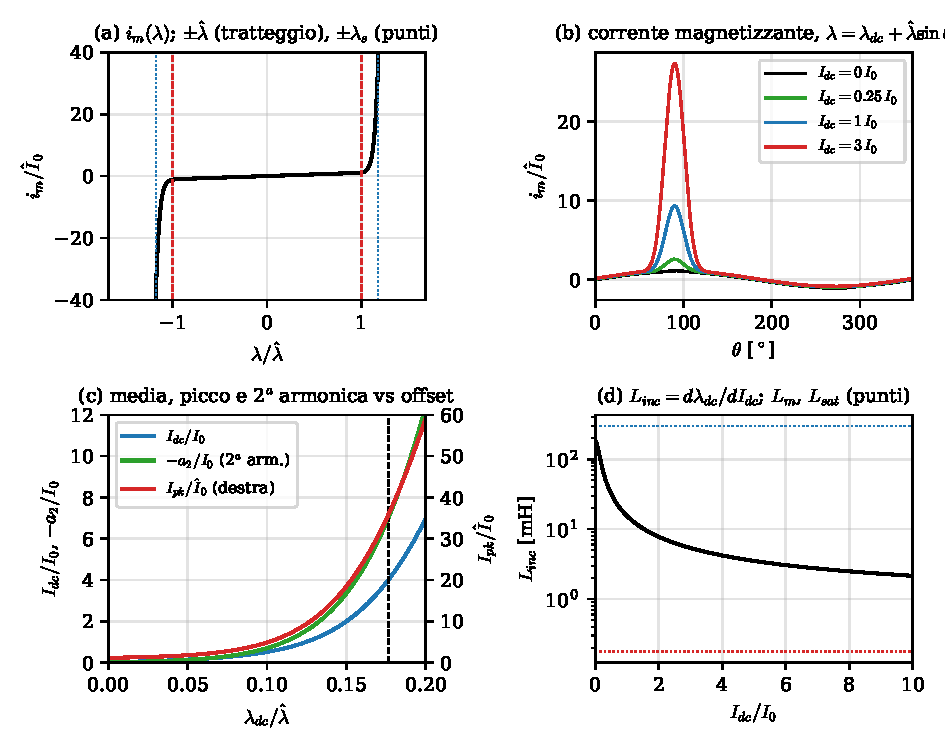
\includegraphics[width=\textwidth]{figures/fig_magnetizing_characteristic.pdf}
\caption{Nucleo senza traferro con offset di flusso ($\Lm = \SI{0.30}{H}$, $\Lsat = \SI{0.18}{mH}$, $\lams/\lamhat = \num{1.18}$). (a) Caratteristica $i_m(\lambda)$. (b) Corrente magnetizzante in un periodo per $\Idc = 0$, $\num{0.25}\,\Izero$, $\Izero$ e $3\,\Izero$: saturazione a semionda. (c) Corrente media, picco dell'impulso e seconda armonica in funzione dell'offset di flusso; il tratteggio è il ginocchio $\lams - \lamhat$. (d) Induttanza incrementale mediata $\dif\lamdc/\dif\Idc$: da $\Lm$ in zona lineare a pochi millihenry in saturazione.}
\label{fig:caratteristica}
\end{figure}

\begin{table}[H]
\centering\small
\begin{tabular}{@{}S[table-format=2.2]S[table-format=2.1]S[table-format=1.3]S[table-format=3.0]S[table-format=2.1]S[table-format=3.1]S[table-format=1.2]S[table-format=3.1]@{}}
\toprule
{$\Idc/\Izero$} & {$\Idc$ [A]} & {$\lamdc/\lamhat$} & {$I_{pk}$ [A]} & {$I_{pk}/\Izeropk$} & {$-a_2$ [A]} & {$-a_2/\Idc$} & {$\Linc$ [mH]} \\
\midrule
0.05 & 0.4 & 0.021 & 14 & 1.3 & 0.3 & 0.77 & 165 \\
0.10 & 0.7 & 0.039 & 16 & 1.5 & 0.6 & 0.86 & 132 \\
0.25 & 1.8 & 0.072 & 27 & 2.6 & 2.1 & 1.11 & 66 \\
0.50 & 3.7 & 0.099 & 50 & 4.7 & 5.0 & 1.35 & 32 \\
1 & 7.4 & 0.125 & 98 & 9.3 & 11.4 & 1.55 & 15.4 \\
2 & 14.8 & 0.150 & 193 & 18.5 & 24.8 & 1.68 & 7.7 \\
3 & 22.2 & 0.165 & 286 & 27.3 & 38.2 & 1.72 & 5.4 \\
5 & 37.0 & 0.186 & 459 & 43.9 & 65.2 & 1.76 & 3.5 \\
10 & 73.9 & 0.217 & 843 & 80.6 & 132.0 & 1.79 & 2.1 \\
\bottomrule
\end{tabular}
\caption{Caratteristica mediata del nucleo con offset di flusso (dati di Tab.~\ref{tab:dati}): offset di flusso, picco dell'impulso magnetizzante, seconda armonica e induttanza incrementale per ogni livello di continua. Il picco dipende dalla rotondità del ginocchio: il modello a due pendenze dà il valore alto.}
\label{tab:caratteristica}
\end{table}

Tre conseguenze della Tab.~\ref{tab:caratteristica} guidano il resto della nota. Primo, già con $\Idc = \Izero$ il picco magnetizzante è dieci volte $\Izeropk$ e con $3\,\Izero$ quasi trenta: l'impulso cresce molto più in fretta della media. Secondo, la seconda armonica è nulla in zona lineare e cresce circa come $\num{1.5}$--$\num{1.8}$ volte la continua oltre il ginocchio: è l'indicatore diagnostico e, in Sez.~\ref{sec:secondaarmonica}, un segnale di retroazione insensibile all'offset dei sensori. Terzo, l'induttanza incrementale mediata scende da $\Lm = \SI{297}{mH}$ a \SI{15}{mH} per $\Idc = \Izero$ e a \SI{5}{mH} per $3\,\Izero$: l'impianto visto da un anello di compensazione cambia di più di cinquanta volte fra nucleo lineare e nucleo saturo (Sez.~\ref{sec:progetto}).

Un nucleo monofase è il caso peggiore: il flusso continuo ha un percorso chiuso interamente nel ferro, come in un nucleo a cinque colonne o corazzato. Un nucleo trifase a tre colonne tollera molto di più, perché il flusso continuo di modo comune deve richiudersi attraverso cassone e aria.

% =====================================================================================================
\section{Effetti della polarizzazione in continua}
\label{sec:effetti}

Il meccanismo di danno è il riscaldamento delle parti strutturali, non del rame. Gli effetti osservabili, in ordine di comparsa:
\begin{itemize}
\item corrente magnetizzante asimmetrica con forte \textbf{seconda armonica} (e armoniche pari in generale): la seconda armonica è l'indicatore diagnostico standard \cite{walling1991};
\item maggiore assorbimento di potenza reattiva, circa proporzionale a $\Idc$;
\item flusso disperso che esce dal nucleo nella semionda satura e si richiude attraverso cassone, pressapacco e piastre di serraggio: \textbf{perdite aggiuntive e punti caldi} nelle parti in acciaio e nel loro isolamento \cite{price2002};
\item \textbf{rumore e vibrazione} in forte aumento (magnetostrizione asimmetrica; \SIrange{10}{20}{dB} con polarizzazione forte);
\item problemi di protezione: un relè differenziale vede un contenuto permanente di seconda armonica, che somiglia a un inrush; l'inverter scatta per sovracorrente sugli impulsi magnetizzanti. Con neutro isolato l'impulso di saturazione di un trasformatore è costretto a richiudersi attraverso gli altri due (Fig.~\ref{fig:forme}, sinistra).
\end{itemize}

% =====================================================================================================
\section{Livello di continua accettabile per un trasformatore monofase da \SI{1.7}{M\VA}}
\label{sec:limiti}

Il limite di continua va riferito alla corrente a vuoto $\Izero$, non alla corrente nominale. Nessuna norma sui trasformatori dà un numero: la IEC 60076 \cite{iec60076} non specifica una tenuta alla continua e la IEEE C57.163 \cite{ieeec57163}, guida per le correnti geomagneticamente indotte, la tratta caso per caso. Per un'unità da \SI{1.7}{M\VA} la corrente a vuoto è tipicamente lo \SIrange{0.2}{0.5}{\percent} di $I_n$.

\begin{table}[H]
\centering\small
\begin{tabular}{@{}R{5.2cm}R{10.3cm}@{}}
\toprule
\textbf{$\Idc$ (sull'avvolgimento che la porta)} & \textbf{Effetto} \\
\midrule
$\lesssim \num{0.1}\,\Izero$ ($\approx \SI{0.03}{\percent}$ di $I_n$) & trascurabile \\
$\approx \Izero$ ($\approx \SI{0.3}{\percent}$ di $I_n$) & saturazione a semionda evidente, picchi magnetizzanti di \numrange{5}{10} volte $\Izero$ secondo la rotondità del ginocchio (Tab.~\ref{tab:caratteristica}), seconda armonica visibile, aumento del rumore \\
$\approx \SI{1}{\percent}$ di $I_n$ ($\approx 3\,\Izero$) & riscaldamento continuo di cassone e serraggi: non accettabile a regime, tollerabile solo come transitorio \\
\bottomrule
\end{tabular}
\caption{Livelli di continua e loro effetto, riferiti alla corrente a vuoto.}
\label{tab:limiti}
\end{table}

Esempio numerico a \SI{690}{V}: $I_n \approx \SI{2460}{A}$, $\Izero \approx \SI{7}{A}$. Sotto circa \SI{1}{A} di continua non si vede nulla; a \SIrange{5}{10}{A} il trasformatore è chiaramente polarizzato; oltre \SIrange{20}{25}{A} continuativi il regime è termicamente dannoso. Su un avvolgimento a tensione più alta le cifre scalano con il rapporto spire: ciò che conta è $N\,\Idc$ confrontato con $N\,\Izero$.

Per riferimento, i limiti di iniezione di continua imposti ai convertitori connessi alla rete, scritti per proteggere i trasformatori di distribuzione, sono lo \SI{0.5}{\percent} di $I_n$ (IEEE 1547 \cite{ieee1547}, CEI 0-21 \cite{cei021}), l'\SI{1}{\percent} (IEC 61727 \cite{iec61727}) e \SI{1}{A} in assoluto (VDE \cite{vde0126}). Anche lo \SI{0.5}{\percent} è paragonabile o superiore alla $\Izero$ di un trasformatore grande: sono compromessi, non valori innocui.

% =====================================================================================================
\section{Resistenza dell'anello in continua e modello nel riferimento \texorpdfstring{$\alpha\beta$}{alfa-beta}}
\label{sec:resistenza}

\subsection{Resistenza vista dall'inverter}

In continua l'inverter vede i trasformatori come un anello di pochi milliohm (Tab.~\ref{tab:resistenza}): ogni \SI{10}{mV} di differenza di tensione continua fra due rami diventano \SIrange{3}{5}{A}, contro una $\Izero$ di circa \SI{7}{A}.

\begin{table}[H]
\centering\small
\begin{tabular}{@{}R{8.5cm}R{6.0cm}@{}}
\toprule
\textbf{Contributo (\SI{690}{V}, \SI{1.7}{M\VA} per fase)} & \textbf{Valore} \\
\midrule
Avvolgimento del trasformatore, perdite nel rame $\approx \SI{1}{\percent}$ & $\approx \SI{2.8}{m\ohm}$ per fase, di cui $\approx \SI{1.4}{m\ohm}$ sul primario \\
Cavi e sbarre & \SIrange{0.5}{1}{m\ohm} \\
Resistenza differenziale di IGBT e diodo (classe \SI{2400}{A}) & $\approx \SI{0.5}{m\ohm}$ \\
Anello totale $R$ & \SIrange{2}{4}{m\ohm}; nel seguito $R = \SI{2.9}{m\ohm}$ \\
\bottomrule
\end{tabular}
\caption{Resistenza dell'anello in continua per fase.}
\label{tab:resistenza}
\end{table}

Ciò che conta è la differenza di tensione continua fra i rami (e fra dispositivo alto e basso dello stesso ramo), non l'errore assoluto di un ramo. Con i primari a stella e neutro isolato le tre correnti continue hanno somma nulla, quindi solo due sono indipendenti, ma ogni trasformatore vede la propria.

\subsection{Il modello in continua è a due gradi di libertà: le componenti \texorpdfstring{$\alpha\beta$}{alfa-beta}}
\label{sec:modelloab}

Siano $v_a$, $v_b$, $v_c$ le tensioni dei rami dell'inverter riferite al punto medio del DC link, $v_n$ quella del centro stella dei primari, $i_k$ le correnti di fase e $\lambda_k$ i flussi concatenati. A vuoto (il secondario non porta continua e a regime non interviene nel bilancio medio)
\begin{equation}
v_k - v_n = R\,i_k + \frac{\dif\lambda_k}{\dif t}, \qquad i_k = i_m(\lambda_k), \qquad i_a + i_b + i_c = 0, \qquad k = a, b, c.
\label{eq:fase}
\end{equation}
A regime periodico il flusso è periodico e la media della sua derivata è nulla: la media su un periodo di \eqref{eq:fase} dà
\begin{equation}
\langle v_k - v_n\rangle = R\,I_k ,
\label{eq:mediafase}
\end{equation}
cioè \emph{la corrente continua di regime è fissata dalla sola resistenza}: il nucleo decide l'offset di flusso e la forma d'onda (Sez.~\ref{sec:semionda}), non la media. Con resistenze uguali, dalla somma nulla delle correnti segue $v_n = (v_a + v_b + v_c)/3$, cioè il centro stella segue la componente omopolare (di modo comune) delle tensioni dei rami, e $v_k - v_n$ è la parte dei $v_k$ a somma nulla.

La trasformata di Clarke invariante in ampiezza \cite{clarke1951}
\begin{equation}
x_\alpha = \tfrac23\left(x_a - \tfrac12 x_b - \tfrac12 x_c\right), \qquad x_\beta = \frac{x_b - x_c}{\sqrt3}, \qquad x_0 = \tfrac13\left(x_a + x_b + x_c\right),
\label{eq:clarke}
\end{equation}
con inversa (senza omopolare) $x_a = x_\alpha$, $x_b = -\tfrac12 x_\alpha + \tfrac{\sqrt3}{2}x_\beta$, $x_c = -\tfrac12 x_\alpha - \tfrac{\sqrt3}{2}x_\beta$, separa esattamente le due parti: $v_n$ è omopolare e sparisce, e \eqref{eq:mediafase} diventa
\begin{equation}
\Iab = \frac{V_{\ab}}{R}, \qquad V_{\ab} = \Eab + \dvab ,
\label{eq:dcab}
\end{equation}
dove $\Eab$ è la componente $\alpha\beta$ dell'errore di tensione continua dell'inverter (Sez.~\ref{sec:sorgenti}) e $\dvab$ l'offset che la compensazione aggiunge al vettore spaziale di riferimento. Due conclusioni:
\begin{itemize}
\item la componente omopolare dell'errore continuo dell'inverter (uguale sui tre rami) non produce corrente: sposta solo il centro stella. L'errore che conta è la sua parte $\alpha\beta$, due numeri;
\item l'inverter può agire solo su $v_\alpha$ e $v_\beta$, ma lo spazio raggiungibile delle correnti continue, con neutro isolato, è esattamente lo spazio $\alpha\beta$: \emph{la limitazione non è una limitazione}. L'annullamento completo delle tre correnti continue si ottiene con $\dvab = -\Eab$, e le tre tensioni di correzione per ramo che ne risultano hanno somma nulla per costruzione. Lo stesso vale per primari a triangolo (le tensioni d'avvolgimento sono concatenate e la somma delle tre è nulla); non vale per una stella con neutro connesso, dove una continua omopolare può circolare e serve un quarto grado di libertà.
\end{itemize}

Con resistenze diverse sulle tre fasi la relazione \eqref{eq:dcab} diventa una matrice $2\times2$: $\Iab = G_{\ab}V_{\ab}$ con $G_{\ab} = T\,(G - g g^{\mathrm T}/\sum_k G_k)\,T^{+}$, $G = \mathrm{diag}(1/R_k)$, $g = [1/R_a\ 1/R_b\ 1/R_c]^{\mathrm T}$, $T$ la Clarke e $T^+$ la sua inversa. Con uno squilibrio del \SI{10}{\percent} ($R_a = \num{1.1}R$, $R_b = \num{0.9}R$) gli elementi diagonali di $R\,G_{\ab}$ sono \num{0.95} e \num{1.05} e quelli fuori diagonale \num{-0.03}; con il \SI{20}{\percent}, \num{0.91}, \num{1.12} e \num{-0.06}. L'accoppiamento fra gli assi è dell'ordine dello squilibrio e non ha effetto su un anello lento con margine di fase ampio (Sez.~\ref{sec:progetto}).

\subsection{Dinamica della componente continua}
\label{sec:dinamica}

La relazione statica \eqref{eq:dcab} non basta a progettare l'anello: la continua raggiunge $V/R$ solo dopo che il flusso si è spostato. Linearizzando \eqref{eq:fase} attorno a un offset, per le componenti lente
\begin{equation}
\Delta v = R\,\Delta i + \Linc\,\frac{\dif\Delta i}{\dif t} \qquad\Longrightarrow\qquad P(s) = \frac{\Delta i}{\Delta v} = \frac{1}{R + s\Linc},
\label{eq:impianto}
\end{equation}
con $\Linc$ l'induttanza incrementale mediata di Fig.~\ref{fig:caratteristica}d, uguale sui due assi perché i trasformatori sono uguali. In zona lineare $\Linc = \Lm$ e la costante di tempo è $\tau_m = \Lm/R = \SI{102}{s}$: a un gradino di errore $E$ la continua risponde come $E\,t/\Lm$, una rampa, e un errore di \SI{67}{mV} porta il flusso al ginocchio in \SI{8.5}{s} (continua di soli \SI{1.8}{A} a quel punto); oltre il ginocchio $\Linc$ cade a \SIrange{5}{15}{mH} (costante di tempo \SIrange{2}{5}{s}) e la continua sale in pochi secondi al valore di regime $E/R = \SI{23}{A}$. A frequenze sopra $R/\Lm = \SI{1.6}{mHz}$ l'impianto in zona lineare è un integratore: questo decide la struttura del regolatore (Sez.~\ref{sec:progetto}).

% =====================================================================================================
\section{Sorgenti di errore in continua dell'inverter in anello aperto}
\label{sec:sorgenti}

Una somma realistica delle sorgenti di Tab.~\ref{tab:sorgenti} è \SIrange{50}{150}{mV} fra i rami, cioè \SIrange{15}{50}{A} di continua su trasformatori con $\Izero \approx \SI{7}{A}$. La saturazione a semionda è dunque l'esito atteso senza compensazione.

\begin{table}[H]
\centering\small
\begin{tabular}{@{}R{4.6cm}R{7.6cm}R{3.0cm}@{}}
\toprule
\textbf{Sorgente} & \textbf{Entità a \SI{1.25}{kHz}, \SI{1070}{V}} & \textbf{Dipende dal carico?} \\
\midrule
Asimmetria temporale alto/basso (ritardi dei gate driver, fibre ottiche, spread di $t_{on}/t_{off}$) & $\Delta V = \Delta t\,\Udc/\Ts \approx \SI{1.34}{V}$ per \si{\micro s}; \SI{50}{ns} $\to$ \SI{67}{mV} $\approx \SI{23}{A}$; \SI{200}{ns} $\to$ \SI{0.27}{V} & no: dominante a vuoto \\
Spread di $V_{ce(sat)}$ / $V_f$ fra dispositivo alto e basso & con dispositivi identici la media si cancella per simmetria; uno spread di \SIrange{\pm 0.1}{\pm 0.3}{V} lascia \SIrange{25}{100}{mV} & sì: piccolo a vuoto \\
Numerica del modulatore (offset della tabella del seno, arrotondamento del confronto, aggiornamento asimmetrico su/giù) & fino a decine di millivolt se non verificata; può essere resa trascurabile & no \\
PWM asincrona (portante non agganciata alla fondamentale) & battimento a $|f_c - 25 f_1|$ con subarmoniche vicine alla continua: il flusso vaga e satura a intermittenza & no \\
\bottomrule
\end{tabular}
\caption{Sorgenti di errore in continua dell'inverter in anello aperto.}
\label{tab:sorgenti}
\end{table}

Il termine temporale è quello da sorvegliare a vuoto. Il termine delle cadute dei dispositivi compare sotto carico ed è il più difficile da prevedere, perché dipende dall'abbinamento reale dei moduli; per l'anello di compensazione è un errore che cambia con il carico e che va inseguito (Sez.~\ref{sec:progetto}).

Esempio usato nelle simulazioni (Sez.~\ref{sec:verifica}): asimmetrie temporali $\Delta t = (+50, -30, +40)\,\si{ns}$ sui tre rami, cioè $E_{abc} = (\num{66.9}, \num{-40.1}, \num{53.5})\,\si{mV}$, con modo comune \SI{26.8}{mV} e parte $\alpha\beta$ $\Eab = (\num{40.1}, \num{-54.0})\,\si{mV}$, $|\Eab| = \SI{67.3}{mV}$. Le correnti continue senza compensazione sono $I_{abc} = (\num{13.8}, \num{-23.1}, \num{9.2})\,\si{A}$, cioè $(\num{1.9}, \num{-3.1}, \num{1.3})\,\Izero$.

% =====================================================================================================
\section{Effetto del tempo morto}
\label{sec:tempomorto}

A \SI{1.25}{kHz} il tempo morto è un errore di tensione grande, ma smorza la componente continua invece di crearla \cite{jeong1991, holmes2003, pwrdeadtime}. Con $t_d = \SI{5}{\micro s}$
\begin{equation}
V_{dt} = \frac{t_d}{\Ts}\,\Udc = \frac{\SI{5}{\micro s}}{\SI{800}{\micro s}}\cdot\SI{1070}{V} \approx \SI{6.7}{V}.
\label{eq:vdt}
\end{equation}
È un'onda quasi quadra in fase con la corrente, $-V_{dt}\,\sign(i)$. Da sola non produce continua, ma un offset nella corrente sposta il rapporto ciclico di $\sign(i)$, e la tensione di tempo morto acquista una componente media che si oppone alla continua: con $i = \hat I\sin\theta + \Idc$ la media di $\sign(i)$ è $(2/\pi)\arcsin(\Idc/\hat I)$ e la resistenza di smorzamento equivalente è
\begin{equation}
R_{eq} \approx \frac{2\,V_{dt}}{\pi\,\hat I},
\label{eq:req}
\end{equation}
cioè circa \SI{1.2}{m\ohm} a $\hat I = \SI{3500}{A}$ e \SI{2.4}{m\ohm} a metà carico. Questo smorzamento gratuito è paragonabile alla resistenza dell'avvolgimento sotto carico, ma non è controllato e cambia con il carico.

A vuoto il comportamento è diverso e vale la pena notarlo: con $\hat I = \Izeropk = \SI{10.5}{A}$ la \eqref{eq:req} non è più una resistenza ma un relè di ampiezza $V_{dt}$ nell'anello in continua, che tiene la continua al valore per cui la corrente cambia ancora segno in quasi metà periodo, $\Idc \approx \Izeropk\,\frac{\pi}{2}\,\frac{E}{V_{dt}} \approx \SI{0.16}{A}$ per $E = \SI{67}{mV}$, finché la commutazione resta dura a queste correnti. Un inverter senza compensazione del tempo morto può quindi \emph{non mostrare} polarizzazione a vuoto e mostrarla sotto carico; con la compensazione del tempo morto attiva questo smorzamento sparisce. Per entrambe le ragioni non va considerato nel progetto, e la verifica al banco deve includere la prova sotto carico (Sez.~\ref{sec:banco}). Le simulazioni di Sez.~\ref{sec:verifica} non includono il tempo morto: è il caso conservativo.

% =====================================================================================================
\section{Energizzazione}
\label{sec:energizzazione}

Un gradino di tensione a frequenza nominale porta il flusso a quasi due volte il picco più la rimanenza: un inrush di decine di kiloampere, limitato solo dall'induttanza satura, e uno scatto per sovracorrente dell'inverter.

Il rimedio in anello aperto è una rampa di tensione da zero a frequenza fissa, lunga \SIrange{0.5}{2}{s}. Il flusso si costruisce allora simmetricamente e l'offset residuo (rimanenza) decade attraverso la resistenza dell'anello e le perdite in zona satura. Con i primari a stella e neutro isolato le tre correnti di inrush sono vincolate a somma nulla e si influenzano a vicenda; la rampa tratta anche questo caso. L'anello di compensazione della continua va attivato dall'inizio della rampa (Sez.~\ref{sec:implementazione}).

% =====================================================================================================
\section{Compensazione della continua sulle componenti \texorpdfstring{$\alpha\beta$}{alfa-beta} del vettore spaziale}
\label{sec:compensazione}

\subsection{Principio}
\label{sec:principio}

Il controllo V/f resta in anello aperto: genera il vettore spaziale di riferimento $v^*_\alpha = \hat V(f)\cos\theta$, $v^*_\beta = \hat V(f)\sin\theta$ con $\theta = \int\omega_1\,\dif t$, e il modulatore (SVM o PWM sinusoidale) lo traduce nei rapporti ciclici dei tre rami. La compensazione è un anello aggiunto che lavora sulla sola componente continua e somma un offset lento al riferimento:
\begin{equation}
v_\alpha^{ref} = v_\alpha^* + \Delta v_\alpha, \qquad v_\beta^{ref} = v_\beta^* + \Delta v_\beta ,
\label{eq:somma}
\end{equation}
con $\dvab$ dell'ordine delle decine o centinaia di millivolt contro un riferimento fondamentale di centinaia di volt: il margine alla sovramodulazione non cambia. L'offset in volt si converte in indice di modulazione con lo stesso guadagno del riferimento fondamentale (per esempio $\Delta m = \Delta v/(\Udc/\sqrt3)$ se $|m| = 1$ è il limite lineare dell'SVM); la componente omopolare che l'SVM aggiunge non interessa la continua, perché il neutro è isolato. La Fig.~\ref{fig:schema} mostra la struttura.

\begin{figure}[H]
\centering
\begin{tikzpicture}[>=Latex, node distance=9mm and 8mm, font=\small,
  blk/.style={draw, rounded corners=1.5pt, minimum height=8mm, minimum width=18mm, align=center, inner sep=3pt},
  sum/.style={draw, circle, minimum size=5mm, inner sep=0pt}]
\node[blk] (vf) {generatore V/f\\$\hat V(f)\,[\cos\theta,\ \sin\theta]$};
\node[sum, right=10mm of vf] (s1) {$+$};
\node[blk, right=10mm of s1] (mod) {modulatore\\SVM / PWM};
\node[blk, right=8mm of mod] (inv) {inverter\\$v_{abc} = v^{ref}_{abc} + e_{abc}$};
\node[blk, right=8mm of inv] (tr) {trafo $a,b,c$\\stella, neutro isolato};
\node[blk, below=12mm of tr] (clk) {Clarke\\$i_{abc} \to i_{\ab}$};
\node[blk, left=8mm of clk] (ma) {media mobile\\su $\Tuno$ ($N_1$ campioni)};
\node[blk, left=8mm of ma] (pi) {PI per asse\\$-(\kp + \ki/s)$, limite $\pm V_{lim}$};
\draw[->] (vf) -- node[above] {$v^*_{\ab}$} (s1);
\draw[->] (s1) -- node[above] {$v^{ref}_{\ab}$} (mod);
\draw[->] (mod) -- node[above] {$d_{abc}$} (inv);
\draw[->] (inv) -- node[above] {$v_{abc}$} (tr);
\draw[->] (tr) -- node[right] {$i_{abc}$ (sensori, $-\hat\delta$)} (clk);
\draw[->] (clk) -- node[above] {$i_{\ab}$} (ma);
\draw[->] (ma) -- node[above] {$\Iab$} (pi);
\draw[->] (pi) -| node[pos=0.25, above] {$\dvab$} (s1);
\node[below=1mm of ma, font=\footnotesize, align=center] {indicatore di 2$^a$ armonica\\in alternativa (Sez.~\ref{sec:secondaarmonica})};
\end{tikzpicture}
\caption{Struttura della compensazione: il V/f resta in anello aperto; la media su un periodo delle correnti di fase, trasformata secondo Clarke, dà il vettore continuo $\Iab$, e un PI per asse aggiunge l'offset $\dvab$ al vettore spaziale di riferimento. $\hat\delta$ è l'offset stimato dei sensori (auto-azzeramento).}
\label{fig:schema}
\end{figure}

\subsection{Dalle tre correnti misurate al vettore continuo}
\label{sec:misura}

La componente continua di ogni corrente di fase è la media su un numero intero di periodi fondamentali. Il modo più semplice ed esatto è la media mobile su un periodo, $N_1 = \Tuno/\Ts$ campioni presi agli istanti di campionamento del controllo ($N_1 = 25$ a \SI{50}{Hz} con un aggiornamento per periodo PWM, 75 a \SI{16.7}{Hz}):
\begin{equation}
\bar I_k[n] = \frac{1}{N_1}\sum_{j=0}^{N_1-1} i_k[n-j], \qquad
H_{ma}(s) \approx \frac{1 - \ee^{-s\Tuno}}{s\Tuno} = \ee^{-s\Tuno/2}\,\frac{\sin(\omega\Tuno/2)}{\omega\Tuno/2}.
\label{eq:mediamobile}
\end{equation}
La media mobile su un periodo ha zeri esatti su tutte le armoniche della fondamentale, compresa la seconda e, con PWM sincrona a rapporto 25, il ripple di commutazione; il suo ritardo di gruppo è $\Tuno/2 = \SI{10}{ms}$, che è il ritardo dominante dell'anello. Se la frequenza varia (rampa di frequenza) $N_1 = \mathrm{round}(\Tuno/\Ts)$ e una frazione di campione di errore lascia nella misura un residuo alla fondamentale dell'ordine di $1/(2N_1)$ della sua ampiezza: non è continua: a carico pieno vale decine di ampere di ondulazione a $f_1$ nella misura, cioè pochi volt di ondulazione sull'uscita del PI, innocua. Un filtro passa-basso del primo ordine non è adeguato: per attenuare la fondamentale a \SI{2460}{A} fino al livello di \SI{1}{A} servirebbe una costante di tempo di decine di secondi.

Poiché la trasformata di Clarke è lineare, la media delle tre correnti e la Clarke commutano: si può calcolare $i_{\ab}$ a ogni passo di controllo, come già avviene nella maggior parte dei codici, e mediare le due componenti. Le due descrizioni sono identiche e il vettore continuo è
\begin{equation}
I_\alpha = \tfrac23\left(\bar I_a - \tfrac12\bar I_b - \tfrac12\bar I_c\right), \qquad I_\beta = \frac{\bar I_b - \bar I_c}{\sqrt3}.
\label{eq:Iab}
\end{equation}
Con somma nulla delle correnti vere, $I_\alpha = \bar I_a$ e $I_\beta = (\bar I_b - \bar I_c)/\sqrt3$; con due soli sensori la terza media è $-(\bar I_a + \bar I_b)$. La parte di modo comune delle tre misure, $\bar I_0 = (\bar I_a + \bar I_b + \bar I_c)/3$, non entra in $\Iab$: con neutro isolato la somma delle correnti vere è nulla, quindi $\bar I_0$ è interamente offset dei sensori e l'anello $\alpha\beta$ lo rigetta per costruzione (Sez.~\ref{sec:offset}).

La misura deve risolvere circa \SI{0.5}{A} di continua su un segnale di \SI{3500}{A} di picco a carico pieno, cioè \SI{1.5e-4}{} del fondo scala: la media su 25 campioni guadagna risoluzione sulla quantizzazione grazie all'ondulazione naturale del segnale, ma un convertitore a 16 bit e un condizionamento con offset stabile sono il requisito reale; l'offset dei sensori è trattato in Sez.~\ref{sec:offset}.

\subsection{Dal vettore continuo all'offset di tensione}
\label{sec:legge}

L'anello agisce per asse, con lo stesso regolatore sui due assi perché l'impianto \eqref{eq:impianto} è uguale sui due:
\begin{equation}
\Delta v_\alpha = -C(s)\,I_\alpha, \qquad \Delta v_\beta = -C(s)\,I_\beta, \qquad C(s) = \kp + \frac{\ki}{s}.
\label{eq:legge}
\end{equation}
Le tre tensioni di correzione per ramo che ne risultano sono l'inversa di Clarke di $\dvab$, a somma nulla:
\begin{equation}
\Delta v_a = \Delta v_\alpha, \qquad \Delta v_b = -\tfrac12\Delta v_\alpha + \tfrac{\sqrt3}{2}\Delta v_\beta, \qquad \Delta v_c = -\tfrac12\Delta v_\alpha - \tfrac{\sqrt3}{2}\Delta v_\beta .
\label{eq:dvabc}
\end{equation}
Componendo \eqref{eq:Iab}, \eqref{eq:legge} e \eqref{eq:dvabc} si ottiene la forma per fase equivalente, $\Delta v_k = -C(s)\,(\bar I_k - \bar I_0)$: l'anello $\alpha\beta$ coincide con tre anelli per fase a cui sia tolta la componente di modo comune della correzione (che non avrebbe effetto) e della misura (che è solo offset). La forma $\alpha\beta$ è quella naturale per il modulatore, che riceve già un vettore spaziale, e rende esplicito che i gradi di libertà sono due.

A regime l'integratore impone $\Iab = 0$ e quindi, per \eqref{eq:dcab}, $\dvab = -\Eab$: l'uscita del compensatore è una misura dell'errore continuo dell'inverter, utile come diagnostica (un valore che cresce nel tempo indica un driver che invecchia o un modulo che scalda in modo asimmetrico).

\subsection{Progetto del regolatore: perché PI e non solo integratore}
\label{sec:progetto}

L'anello aperto, con il ritardo di misura e di attuazione, è
\begin{equation}
L(s) = \left(\kp + \frac{\ki}{s}\right) H_{ma}(s)\,\ee^{-s\,1.5\Ts}\,\frac{1}{R + s\Linc},
\label{eq:anello}
\end{equation}
dove $1.5\Ts = \SI{1.2}{ms}$ è il ritardo di calcolo e di ritenuta della PWM \cite{buso2015}; il ritardo totale è $T_d = \Tuno/2 + 1.5\Ts = \SI{11.2}{ms}$. La difficoltà del progetto è tutta in $\Linc$, che vale $\Lm = \SI{297}{mH}$ in zona lineare e \SIrange{2}{15}{mH} in saturazione (Tab.~\ref{tab:caratteristica}), e l'anello deve essere stabile e ben smorzato in entrambe le condizioni: la zona lineare è quella in cui l'anello deve lavorare a regime, la zona satura è quella in cui si trova alla sua inserzione su un trasformatore già polarizzato o dopo un transitorio.

\textbf{Il solo integratore non basta.} In zona lineare, sopra $R/\Lm = \SI{0.01}{rad/s}$, l'impianto è esso stesso un integratore: con $C(s) = \ki/s$ l'anello è un doppio integratore e il polinomio caratteristico $\Lm s^2 + R s + \ki$ ha smorzamento $\zeta = R/(2\sqrt{\ki\Lm})$, fornito dalla sola resistenza di \SI{2.9}{m\ohm}. Con $\zeta = \num{0.8}$ si ottiene $\ki = \SI{1.1e-5}{V\per(A.s)}$, $\omega_n = \SI{6e-3}{rad/s}$ e un tempo di assestamento di circa \SI{800}{s}; un $\ki$ più alto dà un'oscillazione lenta del flusso. L'intuizione di un anello integrale a \SIrange{0.2}{1}{Hz} funziona solo con il nucleo saturo, dove $\Linc$ è piccola: non è il regime di lavoro.

\textbf{Il termine proporzionale è una resistenza virtuale.} Con $C(s) = \kp + \ki/s$ il polinomio caratteristico in zona lineare diventa
\begin{equation}
\Lm s^2 + (R + \kp)\,s + \ki = 0, \qquad \omega_n = \sqrt{\frac{\ki}{\Lm}}, \qquad \zeta = \frac{R + \kp}{2\sqrt{\ki\Lm}},
\label{eq:caratteristico}
\end{equation}
cioè $\kp$ si somma alla resistenza dell'anello in continua: la sensibilità della continua a un errore di tensione passa da $1/R$ a $1/(R + \kp)$ entro il ritardo della media, e a zero con l'integratore. Per un gradino di errore $E$ la continua resta sotto $E/(R + \kp)$ e, con $\zeta = 1$, raggiunge al massimo $2E/(\ee\,(R + \kp))$. La regola di progetto in zona lineare è
\begin{equation}
\ki = \frac{(R + \kp)^2}{4\zeta^2\Lm}, \qquad \zeta = \numrange{0.8}{1}.
\label{eq:ki}
\end{equation}

\textbf{Il limite di $\kp$ è il nucleo saturo.} In saturazione il guadagno dell'impianto cresce di $\Lm/\Linc$, fino a cinquanta volte e più, e l'attraversamento dell'anello sale a $\omega_c \approx \kp/\Linc$; il margine di fase è eroso dal ritardo $T_d$, $PM \approx 90^\circ - \omega_c T_d$ (in radianti), e per $PM \ge 60^\circ$ serve
\begin{equation}
\kp \le \frac{\num{0.45}\,\Linc^{min}}{T_d} ,
\label{eq:kpmax}
\end{equation}
cioè circa \SI{215}{m\ohm} con $\Linc(3\,\Izero) = \SI{5.4}{mH}$ e \SI{85}{m\ohm} con $\Linc(10\,\Izero) = \SI{2.1}{mH}$. L'induttanza satura assunta ($\Lsat = \SI{0.2}{\pu}$) è il dato più incerto della nota e $\Linc$ scala circa come $\Lsat^{2/3}$ (App.~\ref{app:impulso}): conviene tenersi un fattore due o tre sotto il limite.

La Tab.~\ref{tab:progetto} riporta, per alcuni valori di $\kp$ e con $\ki$ dalla \eqref{eq:ki}, i parametri in zona lineare e i margini di fase ai diversi livelli di saturazione; la Fig.~\ref{fig:bode} mostra l'anello aperto per la scelta di riferimento
\begin{equation}
\kp = \SI{50}{m\ohm} \approx 17\,R, \qquad \ki = \SI{3.7e-3}{V\per(A.s)}, \qquad V_{lim} = \SI{\pm 2}{V},
\label{eq:scelta}
\end{equation}
che dà in zona lineare $\omega_n = \SI{0.11}{rad/s}$ (\SI{18}{mHz}), assestamento in circa \SI{45}{s}, continua massima di \SIrange{0.9}{1.3}{A} per un gradino di \SI{67}{mV} contro \SI{23}{A} senza anello, e margini di fase di $87^\circ$ a $3\,\Izero$ e $79^\circ$ a $10\,\Izero$. Con $\kp = \SI{100}{m\ohm}$ l'assestamento scende a \SI{23}{s} e il picco a \SIrange{0.5}{0.7}{A}, con $64^\circ$ di margine a $10\,\Izero$: è l'alternativa se l'induttanza satura è confermata.

\begin{table}[H]
\centering\small
\begin{tabular}{@{}S[table-format=3.0]S[table-format=2.1]S[table-format=1.1e-1]S[table-format=1.3]S[table-format=3.0]S[table-format=3.1]S[table-format=2.0]S[table-format=3.0]S[table-format=3.0]S[table-format=3.0]@{}}
\toprule
{$\kp$ [m$\Omega$]} & {$\kp/R$} & {$\ki$ [V/(A\,s)]} & {$\omega_n$ [rad/s]} & {$t_{set}$ [s]} & {$I_{pk}/E$ [A/V]} & {PM lin.} & {PM($\Izero$)} & {PM($3\Izero$)} & {PM($10\Izero$)} \\
\midrule
0 & 0 & 1.1e-5 & 0.006 & 820 & 345 & 70 & 89 & 90 & 90 \\
10 & 3.4 & 2.2e-4 & 0.027 & 184 & 77.5 & 74 & 104 & 105 & 104 \\
20 & 6.9 & 6.9e-4 & 0.048 & 104 & 43.7 & 72 & 96 & 96 & 92 \\
50 & 17.2 & 3.7e-3 & 0.111 & 45 & 18.9 & 71 & 90 & 87 & 79 \\
100 & 34.5 & 1.4e-2 & 0.216 & 23 & 9.7 & 70 & 86 & 80 & 64 \\
200 & 69.0 & 5.4e-2 & 0.427 & 12 & 4.9 & 70 & 82 & 68 & 39 \\
\bottomrule
\end{tabular}
\caption{Progetto dell'anello PI con $\ki$ dalla \eqref{eq:ki} ($\zeta = \num{0.8}$) e media mobile su un periodo: pulsazione naturale e tempo di assestamento ($4/(\zeta\omega_n)$) in zona lineare, limite superiore della continua di picco per volt di errore a gradino, margini di fase (gradi) con nucleo lineare e con $\Linc$ a $\Izero$, $3\,\Izero$ e $10\,\Izero$. La prima riga è il solo integratore. I margini sopra $90^\circ$ vengono dall'anticipo dello zero del PI.}
\label{tab:progetto}
\end{table}

\begin{figure}[H]
\centering
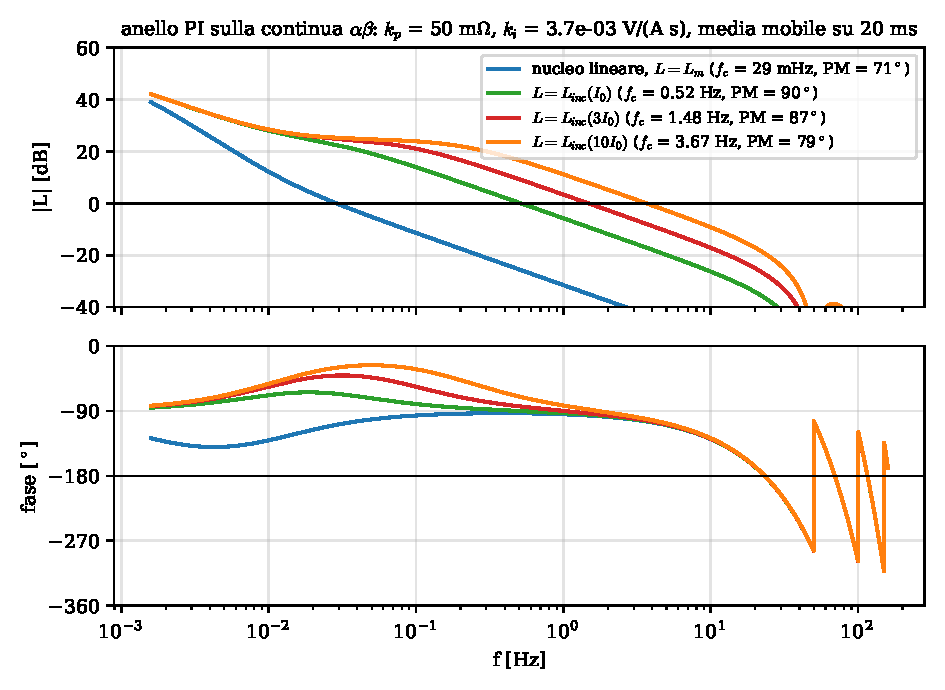
\includegraphics[width=\textwidth]{figures/fig_loop_bode.pdf}
\caption{Anello aperto \eqref{eq:anello} con la scelta \eqref{eq:scelta}, per il nucleo lineare e per tre livelli di saturazione. Lo stesso regolatore attraversa a \SI{29}{mHz} in zona lineare e fino a \SI{3.7}{Hz} con $10\,\Izero$ di continua, sempre con margine di fase sopra $79^\circ$; gli zeri della media mobile sono sulle armoniche di \SI{50}{Hz}.}
\label{fig:bode}
\end{figure}

\subsection{Verifica numerica nel tempo}
\label{sec:verifica}

Lo script simula i tre trasformatori con la caratteristica di Fig.~\ref{fig:caratteristica}a, a stella con neutro isolato e a vuoto (il caso peggiore per la continua: tutta la corrente è magnetizzante), con il modello medio dell'inverter ($v_k = v_k^{ref} + E_k$, senza ripple di commutazione né tempo morto), gli errori $E_{abc}$ di Sez.~\ref{sec:sorgenti}, il controllo campionato a $\Ts = \SI{800}{\micro s}$ e il regolatore \eqref{eq:scelta} in forma discreta (Sez.~\ref{sec:implementazione}); integrazione Runge--Kutta a \SI{100}{\micro s} con proiezione sul vincolo di somma nulla delle correnti. Il flusso parte dal valore di regime, cioè dalla fine di una rampa di avviamento corretta. Quattro scenari (Fig.~\ref{fig:inserzione}--\ref{fig:forme}):

\begin{description}
\item[A, anello inserito a \SI{20}{s}.] Senza compensazione il flusso deriva, la fase $b$ supera il ginocchio a \SI{6.6}{s} e a \SI{20}{s} le continue valgono $(\num{11.5}, \num{-16.8}, \num{5.3})\,\si{A}$, ancora in salita verso il regime $(\num{13.8}, \num{-23.1}, \num{9.2})\,\si{A}$; i picchi di corrente a \SI{15}{s} sono già di \SIlist{129;132;59}{A}, cioè dodici volte $\Izeropk$, con l'impulso della fase satura che si richiude attraverso le altre due (Fig.~\ref{fig:forme}). All'inserzione il termine proporzionale applica subito $\kp\Iab$, circa \SI{0.9}{V}, che desatura il nucleo in meno di un secondo: dopo \SI{1}{s} le continue sono $(\num{2.4}, \num{-4.0}, \num{1.7})\,\si{A}$ e i picchi \SI{20}{A}, dopo \SI{5}{s} $(\num{0.8}, \num{-1.4}, \num{0.6})\,\si{A}$, sotto \SI{0.5}{A} dopo \SI{9}{s} e intorno a \SI{0.1}{A} dopo \SI{20}{s}; l'uscita converge a $\dvab = (\num{-39.5}, \num{53.1})\,\si{mV}$, cioè a $-\Eab$.
\item[B, anello attivo dall'inizio.] La continua non supera \SI{0.9}{A} ($\num{0.12}\,\Izero$, a \SI{8}{s}), l'offset di flusso resta al \SI{39}{\percent} del margine al ginocchio, e la continua scende sotto \SI{0.5}{A} a \SI{20}{s} e sotto \SI{0.2}{A} a \SI{29}{s}. È il funzionamento di progetto: il nucleo non satura mai e l'anello lavora in zona lineare.
\item[C, come B con offset dei sensori $(+5, -2, +4)\,\si{A}$.] Il modo comune (\SI{2.3}{A}) è rigettato; la continua vera di regime è l'opposto della parte differenziale dell'offset, $(\num{-2.7}, \num{4.3}, \num{-1.7})\,\si{A}$: è il limite di Sez.~\ref{sec:offset}.
\item[D, anello di seconda armonica inserito a \SI{20}{s}.] Stessa struttura e stessi guadagni, con l'indicatore di Sez.~\ref{sec:secondaarmonica} al posto della continua misurata: desatura il nucleo (picchi da \SI{130}{A} a \SI{35}{A} in \SI{2}{s}) e porta le continue a $(\num{0.7}, \num{-1.2}, \num{0.6})\,\si{A}$ in \SI{40}{s}, cioè dentro la zona morta dell'indicatore, con una convergenza che rallenta avvicinandosi al ginocchio perché il guadagno dell'indicatore si annulla.
\end{description}

\begin{figure}[!tb]
\centering
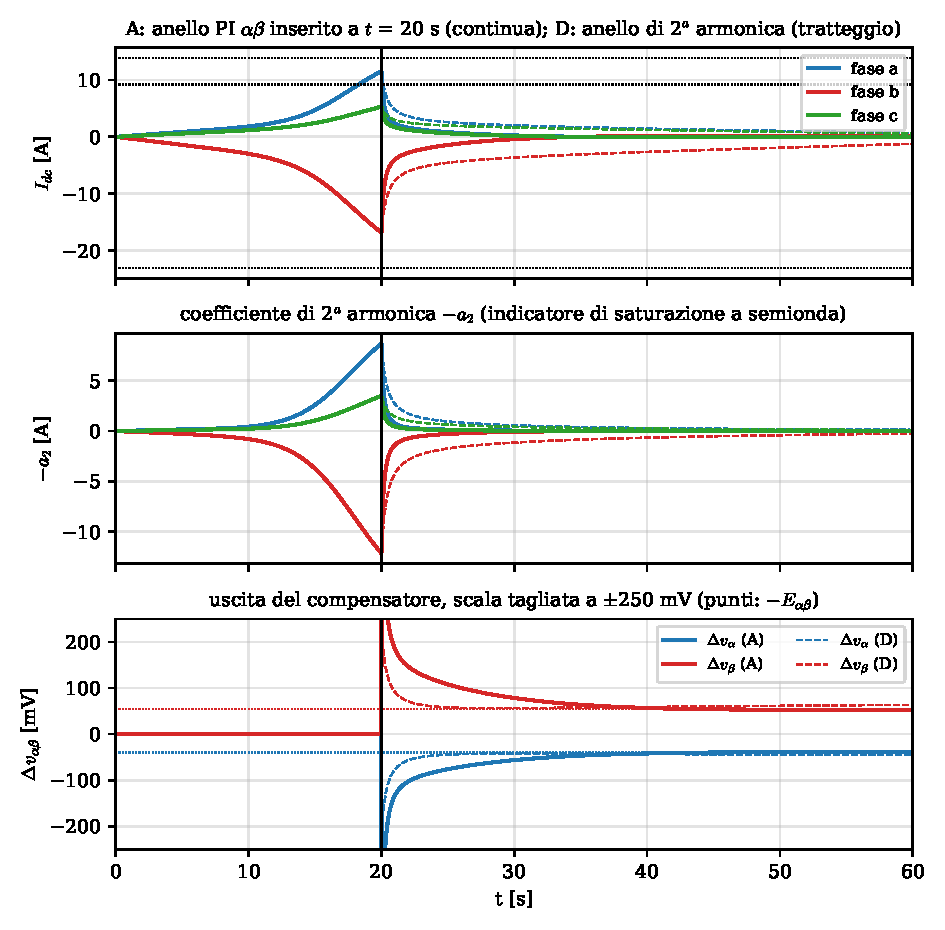
\includegraphics[width=\textwidth]{figures/fig_sim_loop_insertion.pdf}
\caption{Scenario A (linee continue): senza compensazione fino a \SI{20}{s}, poi anello PI $\alpha\beta$; scenario D (tratteggio): anello di seconda armonica. Dall'alto: medie su un periodo delle tre correnti (punti: regime senza compensazione), coefficiente di seconda armonica $-a_2$, uscita del compensatore (punti: $-\Eab$; il picco proporzionale di circa \SI{0.9}{V} all'inserzione è fuori scala).}
\label{fig:inserzione}
\end{figure}

\begin{figure}[!tb]
\centering
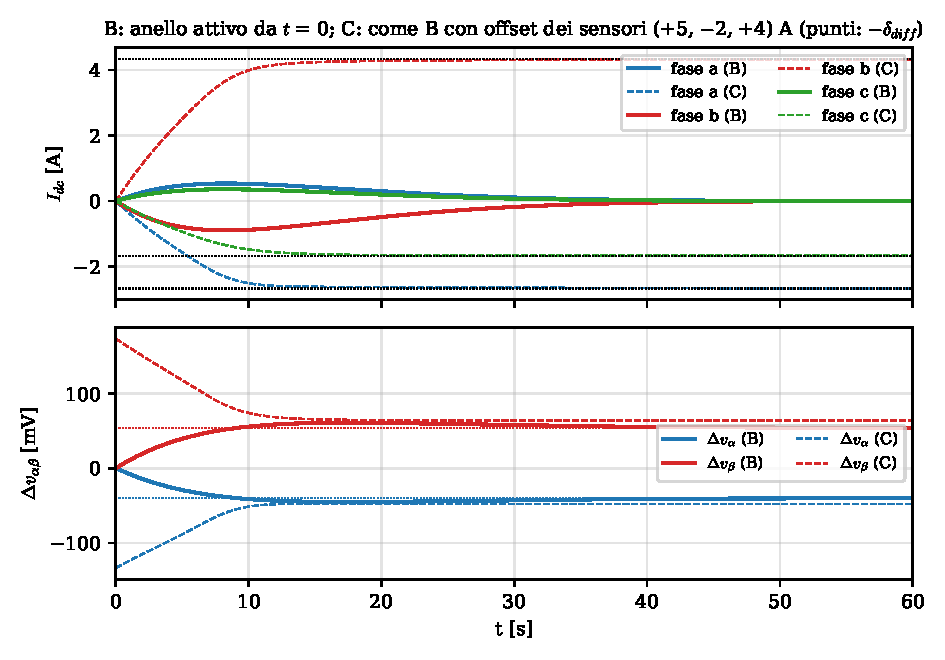
\includegraphics[width=\textwidth]{figures/fig_sim_compensated.pdf}
\caption{Scenario B (linee continue): anello attivo dall'inizio, la continua resta sotto \SI{0.9}{A}; scenario C (tratteggio): stesso anello con offset dei sensori $(+5, -2, +4)\,\si{A}$, la continua vera converge all'opposto della parte differenziale dell'offset (punti) e il modo comune è rigettato.}
\label{fig:compensated}
\end{figure}

\begin{figure}[!tb]
\centering
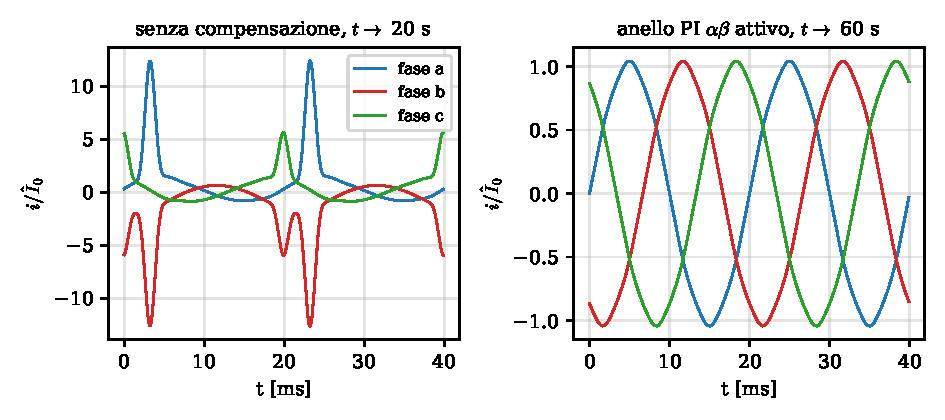
\includegraphics[width=\textwidth]{figures/fig_sim_waveforms.pdf}
\caption{Correnti istantanee in due periodi, in unità di $\Izeropk$. Sinistra: senza compensazione, subito prima dell'inserzione dell'anello (scenario A): la fase $b$ satura nella semionda negativa e il suo impulso si richiude attraverso le fasi $a$ e $c$. Destra: con l'anello attivo a regime, le tre correnti a vuoto sono sinusoidi simmetriche di ampiezza $\Izeropk$.}
\label{fig:forme}
\end{figure}

\subsection{Implementazione discreta}
\label{sec:implementazione}

A ogni passo di controllo $k$ (periodo $\Ts$), per ciascun asse $x \in \{\alpha, \beta\}$:
\begin{equation}
\begin{aligned}
&\text{Clarke delle correnti campionate (offset dei sensori sottratto):} && i_{\ab}[k] = T\,(i_{abc}[k] - \hat\delta_{abc}) \\
&\text{media mobile su un periodo:} && I_x[k] = I_x[k-1] + \tfrac{1}{N_1}\left(i_x[k] - i_x[k-N_1]\right) \\
&\text{errore:} && e_x[k] = 0 - I_x[k] \\
&\text{integratore limitato:} && X_x[k] = \mathrm{sat}\!\left(X_x[k-1] + \ki\Ts\,e_x[k],\ \pm V_{lim}\right) \\
&\text{uscita limitata:} && \Delta v_x[k] = \mathrm{sat}\!\left(\kp\,e_x[k] + X_x[k],\ \pm V_{lim}\right) \\
&\text{riferimento al modulatore:} && v^{ref}_x[k] = v^*_x[k] + \Delta v_x[k].
\end{aligned}
\label{eq:discreto}
\end{equation}
Con i valori \eqref{eq:scelta}, $\ki\Ts = \SI{2.9e-6}{V/A}$ per passo e $\kp = \SI{0.05}{V/A}$; il buffer circolare della media ha $N_1 = 25$ elementi per asse; la media mobile in forma ricorsiva richiede aritmetica che non accumuli errore (interi o doppia precisione), altrimenti va ricalcolata come somma a ogni periodo. Un aggiornamento a ogni passo di controllo, e non una volta per periodo, mantiene il ritardo a $\Tuno/2$; un aggiornamento una volta per periodo aggiungerebbe altri \SI{10}{ms} di ritardo e dimezzerebbe il limite \eqref{eq:kpmax}. Alcune regole pratiche:
\begin{itemize}
\item \textbf{abilitazione:} l'anello è attivo dal primo passo della rampa di avviamento e congelato (integratore mantenuto, uscita mantenuta) quando la modulazione è bloccata o durante uno scatto; la media mobile va azzerata alla ripartenza;
\item \textbf{precarico:} l'errore continuo dell'inverter è ripetibile (asimmetrie temporali, abbinamento dei moduli): memorizzare $X_{\ab}$ allo spegnimento e precaricarlo alla ripartenza accorcia il transitorio a pochi secondi;
\item \textbf{limite e allarme:} $V_{lim} = \SI{2}{V}$ copre trenta volte l'errore atteso; un'uscita che raggiunge il limite segnala un sensore guasto o un offset non azzerato e deve generare un allarme, non una correzione;
\item \textbf{diagnostica:} $|\Iab|$ e $\dvab$ vanno registrati; una continua misurata oltre $\Izero$ per più di dieci secondi con l'anello attivo è un'anomalia (anello aperto, sensore, saturazione per altra causa);
\item \textbf{frequenza di uscita diversa:} a \SI{16.7}{Hz} il periodo è \SI{60}{ms} e il ritardo della media \SI{30}{ms}, e flusso, $\Lm$ e $\Linc$ cambiano con il progetto del trasformatore: $\kp$ va ridotto per lo stesso margine \eqref{eq:kpmax} e $\ki$ ricalcolata con la \eqref{eq:ki}; lo script lo fa cambiando $f_1$ e i dati del trasformatore.
\end{itemize}

\subsection{Offset dei sensori di corrente}
\label{sec:offset}

L'offset dei sensori è il fattore limitante dell'anello e va trattato esplicitamente: a regime l'integratore annulla la continua \emph{misurata}, quindi la continua vera è l'opposto dell'offset. Un sensore a effetto Hall con portata di \SIrange{3}{5}{kA} ha un offset dello \SIrange{0.1}{0.5}{\percent}, cioè \SIrange{3}{25}{A}: esattamente la continua che l'anello inietterebbe.
\begin{itemize}
\item \textbf{Modo comune rigettato.} L'anello usa solo $\Iab$: un offset uguale sui tre sensori (stessa deriva termica di tre sensori uguali) non ha effetto; conta la parte differenziale $\delta_k - \bar\delta$ (scenario C).
\item \textbf{Auto-azzeramento} con l'inverter fermo, prima di ogni avviamento: elimina l'offset iniziale; resta la deriva termica durante il funzionamento, che per sensori Hall a compensazione di flusso vale tipicamente alcuni ampere riportati al primario sull'intervallo di temperatura.
\item \textbf{Sensori flux-gate} (classe LEM IT/ITN) dove il budget lo consente: offset e deriva di uno o due ordini di grandezza più bassi, sufficienti per il target di $\num{0.1}\,\Izero$.
\item \textbf{Regolazione della seconda armonica} (Sez.~\ref{sec:secondaarmonica}): insensibile all'offset, da sola o come correttore lento dell'offset stimato $\hat\delta$ dell'anello principale.
\end{itemize}

\subsection{Alternativa insensibile all'offset: regolazione della seconda armonica}
\label{sec:secondaarmonica}

La seconda armonica della corrente di fase compare solo con saturazione asimmetrica e non dipende dall'offset dei sensori (un offset è continua, non seconda armonica). La sua fase rispetto alla fondamentale dà il segno della correzione. Con il riferimento di fase $v^*_k = \hat V\cos\theta_k$, $\theta_k = \theta - 2\pi k/3$, il flusso è $\lambda_k = \lamhat\sin\theta_k$: un offset positivo satura attorno a $\theta_k = \pi/2$, dove $\cos 2\theta_k = -1$, e l'impulso di corrente ha coefficiente coseno della seconda armonica $a_2 < 0$ (circa $-2\,I_{exc}$, App.~\ref{app:impulso}); un offset negativo dà l'impulso opposto attorno a $3\pi/2$ e $a_2 > 0$. La demodulazione sincrona con il coseno del doppio dell'angolo di riferimento,
\begin{equation}
a_{2,k} = \frac{2}{N_1}\sum_{j=0}^{N_1-1} i_k[n-j]\cos\!\left(2\theta_k[n-j]\right), \qquad \iota_k = -\frac{a_{2,k}}{g_2}, \qquad g_2 \approx 2 ,
\label{eq:demod}
\end{equation}
dà un indicatore $\iota_k$ che è nullo in zona lineare, ha il segno della continua e, oltre il ginocchio, vale circa la corrente in eccesso $\Idc - \lamdc/\Lm$ (Tab.~\ref{tab:caratteristica}: $-a_2/\Idc$ tende a \num{1.8}). La fondamentale, le armoniche dispari e il ripple sincrono si mediano a zero su un periodo; un termine in seno, $\sin 2\theta_k$, è nullo per simmetria dell'impulso e può servire come controllo di coerenza (resta piccolo solo se l'angolo di riferimento e il verso dei sensori sono corretti: il segno va verificato al banco).

L'indicatore entra nella stessa struttura $\alpha\beta$: Clarke dei tre $\iota_k$, PI per asse con gli stessi guadagni, offset $\dvab$ sul riferimento. Le differenze rispetto all'anello sulla continua misurata sono due. L'indicatore ha una \emph{zona morta}: è nullo finché il nucleo non satura (nel modello, $|a_2| < \num{0.1}\,\Izero$ per $\Idc < \num{0.11}\,\Izero$, e il guadagno diventa pieno oltre $\num{0.5}\,\Izero$), quindi l'anello regola la continua alla soglia di saturazione e non a zero, e in zona lineare è aperto: il residuo è dell'ordine di \SIrange{0.5}{2}{A}, cioè il livello a cui la polarizzazione è per definizione invisibile. E la convergenza rallenta avvicinandosi al ginocchio (scenario D). È il regolatore giusto se i sensori sono Hall e la loro deriva supera il residuo accettabile; con sensori buoni l'anello sulla continua è più rapido e porta a zero. La combinazione è naturale: anello principale sulla continua misurata, e indicatore di seconda armonica che corregge lentamente la stima $\hat\delta_{\ab}$ dell'offset dei sensori (una costante di tempo di minuti basta, perché la deriva termica è lenta), così che la continua vera resti sotto la soglia di saturazione anche quando l'offset deriva. Il metodo è nello spirito dei rilevatori di polarizzazione basati sull'asimmetria della corrente magnetizzante \cite{buticchi2013} e delle compensazioni per inverter con trasformatore \cite{buticchi2011, blewitt2010}.

\subsection{Altre contromisure}
\label{sec:altre}

\begin{enumerate}
\item \textbf{PWM sincrona.} Agganciare la portante alla fondamentale con rapporto di impulsi fisso 25; se $f_{sw}$ può essere scelta, 21 o 27 (multipli dispari di 3) danno pattern identici sulle tre fasi; evita le subarmoniche del battimento e rende esatta la media su un periodo.
\item \textbf{Compensazione del tempo morto}, gate driver con ritardi alto/basso accoppiati, e verifica del modulatore per l'offset numerico (tabella del seno, arrotondamento del confronto, simmetria dell'aggiornamento): riducono l'errore $\Eab$ alla sorgente e quindi il lavoro dell'anello, ma non lo sostituiscono, perché lo spread delle cadute dei dispositivi resta.
\item \textbf{Rampa di tensione all'avviamento} (Sez.~\ref{sec:energizzazione}), con l'anello attivo dal primo passo.
\end{enumerate}

% =====================================================================================================
\section{Verifica al banco}
\label{sec:banco}

Misurare con sensori di corrente che passano la continua (Hall o flux-gate, non TA), prima a vuoto e poi sotto carico; la prova a vuoto da sola può non mostrare la polarizzazione (Sez.~\ref{sec:tempomorto}).
\begin{itemize}[label=$\square$]
\item media di ogni corrente di fase su $N$ periodi fondamentali ($N \ge 10$), con auto-azzeramento dei sensori fatto prima della prova;
\item contenuto di seconda armonica di ogni corrente di fase (FFT o demodulazione sincrona \eqref{eq:demod}), e segno di $a_2$ rispetto al segno della media: fissa il segno dell'indicatore;
\item picco positivo contro picco negativo della corrente a vuoto di ogni trasformatore;
\item corrente a vuoto a tensione nominale confrontata con la $\Izero$ attesa; dalla stessa prova, con una continua nota iniettata dall'anello ($\dvab$ imposto), la resistenza dell'anello $R = |\dvab|/|\Iab|$ e, dal transitorio, $\Linc$;
\item con l'anello attivo: $\dvab$ di regime (misura dell'errore dell'inverter) a vuoto e a carico, e risposta all'inserzione su trasformatore polarizzato;
\item rumore udibile a vuoto come indicatore qualitativo di polarizzazione;
\item temperatura di cassone e struttura di serraggio dopo qualche ora a vuoto e a carico;
\item corrente di inrush durante la rampa di avviamento.
\end{itemize}

% =====================================================================================================
\section{Punti aperti}
\label{sec:aperti}

I numeri della nota cambiano con i dati seguenti, ancora da confermare:
\begin{itemize}[label=$\square$]
\item tensione nominale dell'avvolgimento primario e se \SI{1.7}{M\VA} è per unità o totale (fissa $I_n$, $\Izero$, $\Lm$ e la resistenza dell'anello). Con avvolgimenti da \SI{398}{V} a stella sui \SI{690}{V} concatenati e \SI{1.7}{M\VA} per unità: $I_n = \SI{4270}{A}$, $\Izero = \SI{12.8}{A}$, $\Lm = \SI{0.10}{H}$, $R \approx \SI{2.0}{m\ohm}$ (\SI{10}{mV} $\to$ \SI{5}{A}), $\tau_m = \SI{50}{s}$, $\Lsat = \SI{0.06}{mH}$: il limite \eqref{eq:kpmax} su $\kp$ si abbassa di circa tre volte;
\item collegamento dei primari: stella con neutro isolato, stella con neutro, o triangolo (Sez.~\ref{sec:modelloab});
\item frequenza di uscita (\SI{50}{Hz} assunti; a \SI{16.7}{Hz} il rapporto di impulsi diventa 75, Sez.~\ref{sec:implementazione});
\item corrente a vuoto, perdite nel rame e, se disponibile, induttanza satura o corrente di inrush dei trasformatori (rapporto di prova): $\Lsat$ fissa il limite su $\kp$;
\item tempo morto e ritardi dei gate driver dell'inverter;
\item tipo, portata e offset dei sensori di corrente disponibili per l'anello; numero di bit del convertitore;
\item istante e periodo di campionamento del controllo (un aggiornamento per periodo PWM assunto; con doppio aggiornamento $N_1 = 50$ e $\Ts = \SI{400}{\micro s}$).
\end{itemize}

% =====================================================================================================
\appendix
\section{Approssimazioni chiuse per l'impulso di saturazione}
\label{app:impulso}

Con la caratteristica a due pendenze e ginocchio netto, $i_m = \lambda/\Lm$ per $|\lambda| < \lams$ e pendenza $1/\Lsat$ oltre, sia $x = \lamdc - (\lams - \lamhat) > 0$ l'offset oltre il ginocchio. Il nucleo è saturo dove $\lamhat\sin\theta > \lamhat - x$, cioè in un intervallo di semiampiezza $\delta \approx \sqrt{2x/\lamhat}$ attorno a $\theta = \pi/2$ (per $x \ll \lamhat$), dove $\lambda - \lams \approx x - \lamhat(\theta - \pi/2)^2/2$. La corrente in eccesso ha media, picco e induttanza incrementale
\begin{equation}
I_{exc} \approx \frac{2\sqrt2}{3\pi}\,\frac{x^{3/2}}{\Lsat\sqrt{\lamhat}}, \qquad
I_{pk} \approx \frac{x}{\Lsat}, \qquad
\Linc = \frac{\dif x}{\dif I_{exc}} \approx \frac{\pi}{\sqrt2}\,\Lsat\sqrt{\frac{\lamhat}{x}} ,
\label{eq:impulso}
\end{equation}
quindi $I_{pk}/I_{exc} \approx \frac{3\pi}{2\sqrt2}\sqrt{\lamhat/x}$: il rapporto fra picco e media cresce al diminuire dell'offset, e per $x/\lamhat = \num{0.05}$ vale circa 15. Invertendo la prima, $x \propto (I_{exc}\Lsat)^{2/3}$ e $\Linc \propto \Lsat^{2/3}$ a corrente continua fissata: un'induttanza satura dimezzata riduce $\Linc$ di \SI{37}{\percent}. Lo sviluppo in serie dell'impulso, stretto e centrato in $\pi/2$, ha coefficiente coseno dell'armonica $h$ pari a $(1/\pi)\int p\,\cos h\theta\,\dif\theta \approx 2\,I_{exc}\cos(h\pi/2)$: la seconda armonica è $a_2 \approx -2\,I_{exc}$, la quarta $+2\,I_{exc}$, le dispari nulle. Il ginocchio arrotondato usato nello script ($w = \num{0.03}\,\lamhat$) anticipa l'asimmetria e dà $-a_2/\Idc$ da \num{0.8} a \num{1.8} (Tab.~\ref{tab:caratteristica}).

\section{Script di accompagnamento}
\label{app:script}

\code{dc\_bias\_analysis.py} (Python~3, numpy, matplotlib; circa tre minuti per le simulazioni) stampa ogni numero della nota nell'ordine delle sezioni e scrive le figure in \code{figures/}: dati e grandezze derivate, anche per l'avvolgimento da \SI{398}{V}; bilancio delle sorgenti di errore e tempo morto; caratteristica mediata (Tab.~\ref{tab:caratteristica}, Fig.~\ref{fig:caratteristica}); matrice di conduttanza $\alpha\beta$ con resistenze squilibrate; tabella di progetto e Bode dell'anello (Tab.~\ref{tab:progetto}, Fig.~\ref{fig:bode}); simulazione dei quattro scenari (Fig.~\ref{fig:inserzione}--\ref{fig:forme}). I dati di testa (tensione e potenza dell'avvolgimento, corrente a vuoto, perdite, induzioni, $\Lsat$, frequenza, DC link, frequenza di commutazione, tempo morto, resistenze esterne) sono le variabili delle prime righe.

\end{onehalfspace}

\begin{thebibliography}{99}
\small
\bibitem{iec60076} IEC 60076-1:2011, \emph{Power transformers -- Part 1: General}. IEC, Geneva, 2011.
\bibitem{ieeec57163} IEEE Std C57.163-2015, \emph{IEEE Guide for Establishing Power Transformer Capability while under Geomagnetic Disturbances}. IEEE, 2015.
\bibitem{walling1991} R.~A. Walling and A.~N. Khan, ``Characteristics of transformer exciting-current during geomagnetic disturbances,'' \emph{IEEE Trans. Power Del.}, vol.~6, no.~4, pp.~1707--1714, Oct. 1991.
\bibitem{price2002} P.~R. Price, ``Geomagnetically induced current effects on transformers,'' \emph{IEEE Trans. Power Del.}, vol.~17, no.~4, pp.~1002--1008, Oct. 2002.
\bibitem{ieee1547} IEEE Std 1547-2018, \emph{IEEE Standard for Interconnection and Interoperability of Distributed Energy Resources with Associated Electric Power Systems Interfaces}. IEEE, 2018.
\bibitem{cei021} CEI 0-21, \emph{Regola tecnica di riferimento per la connessione di Utenti attivi e passivi alle reti BT delle imprese distributrici di energia elettrica}. CEI, Milano.
\bibitem{iec61727} IEC 61727:2004, \emph{Photovoltaic (PV) systems -- Characteristics of the utility interface}. IEC, Geneva, 2004.
\bibitem{vde0126} DIN V VDE V 0126-1-1, \emph{Automatic disconnection device between a generator and the public low-voltage grid}. VDE, Berlin.
\bibitem{clarke1951} W.~C. Duesterhoeft, M.~W. Schulz, and E.~Clarke, ``Determination of instantaneous currents and voltages by means of alpha, beta, and zero components,'' \emph{Trans. AIEE}, vol.~70, no.~2, pp.~1248--1255, 1951.
\bibitem{jeong1991} S.-G. Jeong and M.-H. Park, ``The analysis and compensation of dead-time effects in PWM inverters,'' \emph{IEEE Trans. Ind. Electron.}, vol.~38, no.~2, pp.~108--114, Apr. 1991.
\bibitem{holmes2003} D.~G. Holmes and T.~A. Lipo, \emph{Pulse Width Modulation for Power Converters: Principles and Practice}. IEEE Press / Wiley, 2003.
\bibitem{pwrdeadtime} pwr-control, \emph{Dead time in voltage source converters}, nota \path{research/power_electronics/dead_time} del repository repositories-documentation.
\bibitem{buso2015} S.~Buso and P.~Mattavelli, \emph{Digital Control in Power Electronics}, 2nd ed. Morgan \& Claypool, 2015.
\bibitem{buticchi2011} G.~Buticchi, E.~Lorenzani, and G.~Franceschini, ``A DC offset current compensation strategy in transformer-based grid-connected inverters,'' \emph{IEEE Trans. Power Del.}, vol.~26, no.~4, pp.~2743--2751, Oct. 2011.
\bibitem{buticchi2013} G.~Buticchi and E.~Lorenzani, ``Detection method of the DC bias in distribution power transformers,'' \emph{IEEE Trans. Ind. Electron.}, vol.~60, no.~8, pp.~3539--3549, Aug. 2013.
\bibitem{blewitt2010} W.~M. Blewitt, D.~J. Atkinson, J.~Kelly, and R.~A. Lakin, ``Approach to low-cost prevention of DC injection in transformerless grid-connected inverters,'' \emph{IET Power Electron.}, vol.~3, no.~1, pp.~111--119, Jan. 2010.
\end{thebibliography}

\end{document}
